% \documentclass[aspectratio=169,notes]{beamer}
\documentclass[aspectratio=169]{beamer}
\usetheme[faculty=phil]{fibeamer}
\usepackage{polyglossia}
\setmainlanguage{english} %% main locale instead of `english`, you
%% can typeset the presentation in either Czech or Slovak,
%% respectively.
\setotherlanguages{russian} %% The additional keys allow
%%
%%   \begin{otherlanguage}{czech}   ... \end{otherlanguage}
%%   \begin{otherlanguage}{slovak}  ... \end{otherlanguage}
%%
%% These macros specify information about the presentation
\title[IME]{Introduction to Mechanical Engineering, HW CAE DYN 2} %% that will be typeset on the
\subtitle{Motion Analysis
\\ \  \\ \ 
         } %% title page.
\author{Oleg Bulichev}
%% These additional packages are used within the document:
\usepackage{ragged2e}  % `\justifying` text
\usepackage{booktabs}  % Tables
\usepackage{tabularx}
\usepackage{tikz}      % Diagrams
\usetikzlibrary{calc, shapes, backgrounds}
\usepackage{amsmath, amssymb}
\usepackage{url}       % `\url`s
\usepackage{listings}  % Code listings
% \usepackage{subfigure}
\usepackage{floatrow}
\usepackage{subcaption}
\usepackage{mathtools}
\usepackage{todonotes}
\usepackage{fontspec}
\usepackage{multicol}
\usepackage{pdfpages}
\usepackage{wrapfig}
\usepackage{animate}
\usepackage{booktabs}
\usepackage{multirow}
% \usepackage{graphicx}
\usepackage{colortbl}

\graphicspath{{resources/}}
\frenchspacing

\setbeamertemplate{caption}[numbered]
\usetikzlibrary{graphs}

% \usepackage[backend=biber,style=ieee,autocite=footnote]{biblatex}
% \addbibresource{biblio.bib}
% \DefineBibliographyStrings{english}{%
%   bibliography = {References},}

\newcommand{\oleg}[2][] {\todo[color=red, #1] {OLEG:\\ #2}}
\newcommand{\fbckg}[1]{\usebackgroundtemplate{\includegraphics[width=\paperwidth]{#1}}}%frame background

\usepackage[framemethod=TikZ]{mdframed}
\newcommand{\dbox}[1]{
\begin{mdframed}[roundcorner=3pt, backgroundcolor=yellow, linewidth=0]
\vspace{1mm}
{#1}
\vspace{1mm}
\end{mdframed}
}

\begin{document}
\setlength{\abovedisplayskip}{0pt}
\setlength{\belowdisplayskip}{0pt}
\setlength{\abovedisplayshortskip}{0pt}
\setlength{\belowdisplayshortskip}{0pt}

\fbckg{fibeamer/figs/title_page.png}
\frame[c]{\setcounter{framenumber}{0}
    \usebeamerfont{title}%
    \usebeamercolor[fg]{title}%
    \begin{minipage}[b][6.5\baselineskip][b]{\textwidth}%
        \textcolor{black}{\raggedright\inserttitle}
    \end{minipage}
    % \vskip-1.5\baselineskip

    \usebeamerfont{subtitle}%
    \usebeamercolor[fg]{framesubtitle}%
    \begin{minipage}[b][3\baselineskip][b]{\textwidth}
        \raggedright%
        \insertsubtitle%
    \end{minipage}
    \vskip.25\baselineskip
}
%   \frame[c]{\maketitle}

\fbckg{fibeamer/figs/common.png}

\note{\scriptsize \begin{itemize}
        \item \
    \end{itemize}}

\note{
    \
}

\begin{frame}[t]{Short Task Description}
    \framesubtitle{}
    \textbf{Description}: Solve 4 tasks, using Motion Analysis NX application

    \textbf{Zip archive, which contains all needed data}: \textit{HWs/HW\_CAE\_DYN2/task\_data}

    \textbf{Artifacts}:
    \begin{itemize}
        \item Zip archive with NX detail files (.prt) and simulation (.sim) for each task in separate folder.
        \item Plots and answers (if particular task requires) in pdf format (.pdf). It should be put in the task folder.
    \end{itemize}
\end{frame}

\begin{frame}[t]{Task 1}
    \framesubtitle{Extended Task Description}
    \textbf{Goal}: \begin{enumerate}
        \item Make a simulation, which repeats the video from the next slide.
        \item Draw 2 plots $x(t)$, $y(t)$ for the center of a green disk in absolute coordinate frame. It can be done, adding a marker into the center of the disk.
        \item Make a plot $R_z(t)$ for a center of disk relative to a right bottom corner of \textit{OSNOVA\_DLIN}. It can be done by sensor and marker.
    \end{enumerate}
    \smallskip

    \textbf{Description}: You don't need to add any drivers. 
\end{frame}

\begin{frame}[t]{Task 1}
    \framesubtitle{Video}
    \vspace{-0.6cm}
    \begin{figure}[H]
        \href{https://disk.yandex.ru/i/-vrZe2tMoOiVMQ}{
            \centering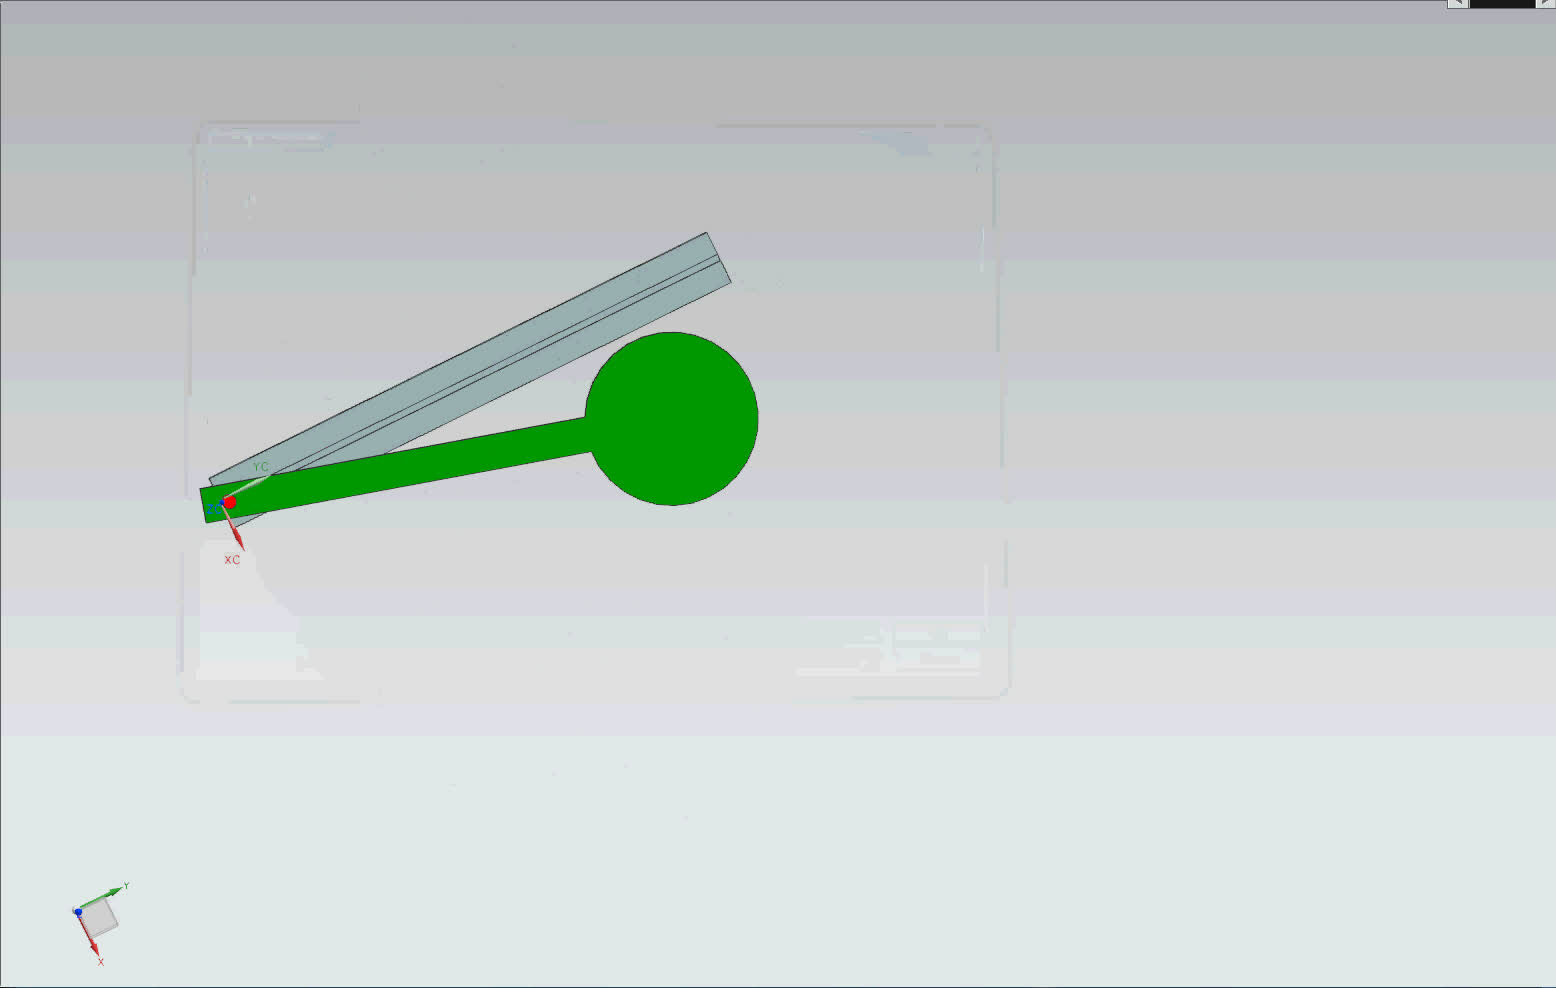
\includegraphics[height=6cm,width=1\textwidth,keepaspectratio]{1_preview.png}}
        % \caption{Click on a picture for a video}
        \label{fig:1_preview.png}
    \end{figure}
\end{frame}


\begin{frame}[t]{Task 2}
    \framesubtitle{Extended Task Description}
    \textbf{Goal}: Make a simulation, which repeats the video from the next slide.
    \smallskip

    \textbf{Description}: To do this, it is recommended that two, time-differentiated forces of 0.5 $N$ and 1 $N$ be applied to the puck. The puck must hit the goal.

    \textbf{Hint}: I used trace for choosing direction of the second force (second puck in the video).
\end{frame}

\begin{frame}[t]{Task 2}
    \framesubtitle{Video}
    \vspace{-0.6cm}
    \begin{figure}[H]
        \href{https://disk.yandex.ru/i/iwNthKk0RIUtEg}{
            \centering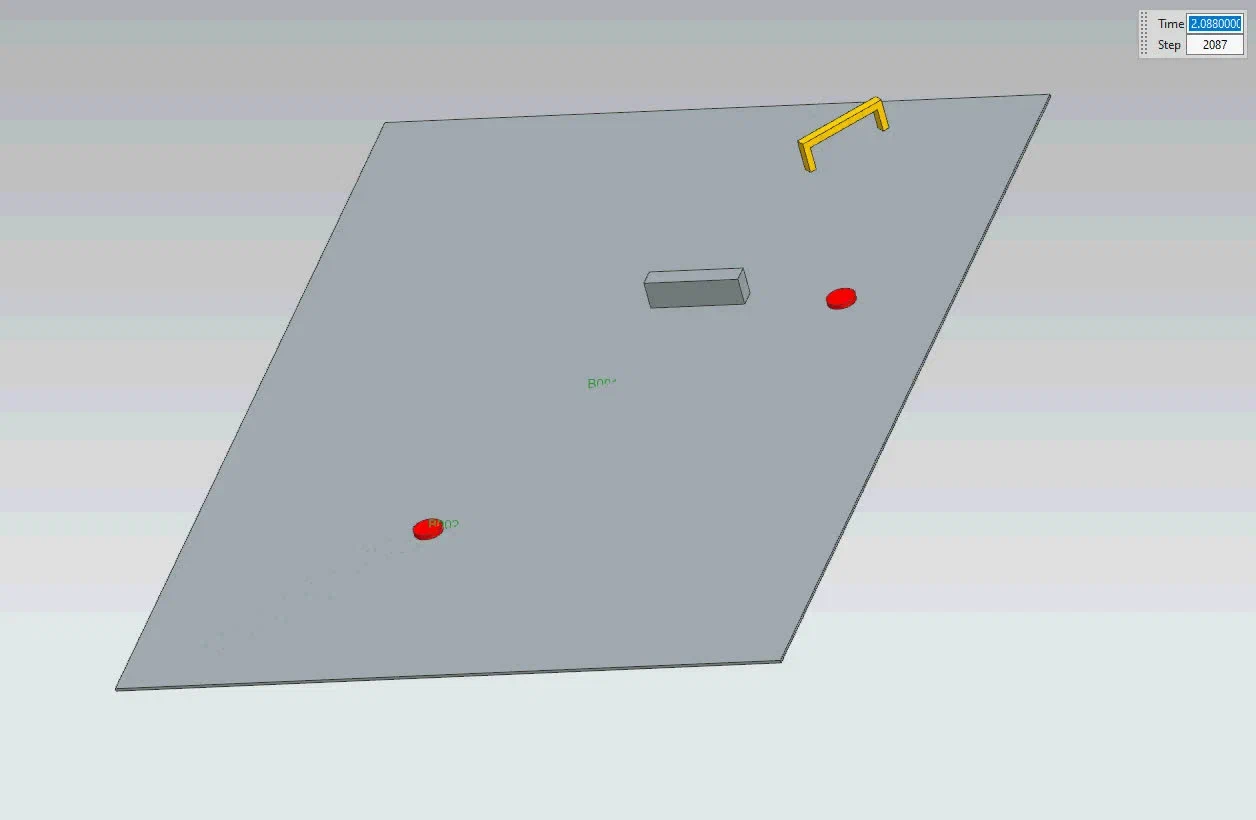
\includegraphics[height=6cm,width=1\textwidth,keepaspectratio]{2_preview.png}}
        % \caption{Click on a picture for a video}
        \label{fig:2_preview.png}
    \end{figure}
\end{frame}

\begin{frame}[t]{Task 3}
    \framesubtitle{Extended Task Description}
    \vspace{-0.5cm}
    \textbf{Goal}: \begin{enumerate}
        \item Make a simulation, which almost repeats the video from the next slide.
        \item Firstly, determine only a stiffness for a spring. Make a plot $Z(t)$ for a corner of a crank.
        \item Add a damper to a string. Make a plot $Z(t)$ for a corner of a crank.
        \item Find a static equilibrium solution (using static analysis solver). If it doesn't work, change the stiffness or damping until it does.
        \item Draw plots of needed (your own thoughts) reaction forces and torques, using "Load Transfer" function.
    \end{enumerate}
    
    
    \smallskip

    \textbf{Description}: same weight of loads, one part of the scale should be connected by spherical joint, another one --- using spring.  
\end{frame}

\begin{frame}[t]{Task 3}
    \framesubtitle{Video}
    \vspace{-0.6cm}
    \begin{figure}[H]
        \href{https://disk.yandex.ru/i/Hw4DpScaAzPctg}{
            \centering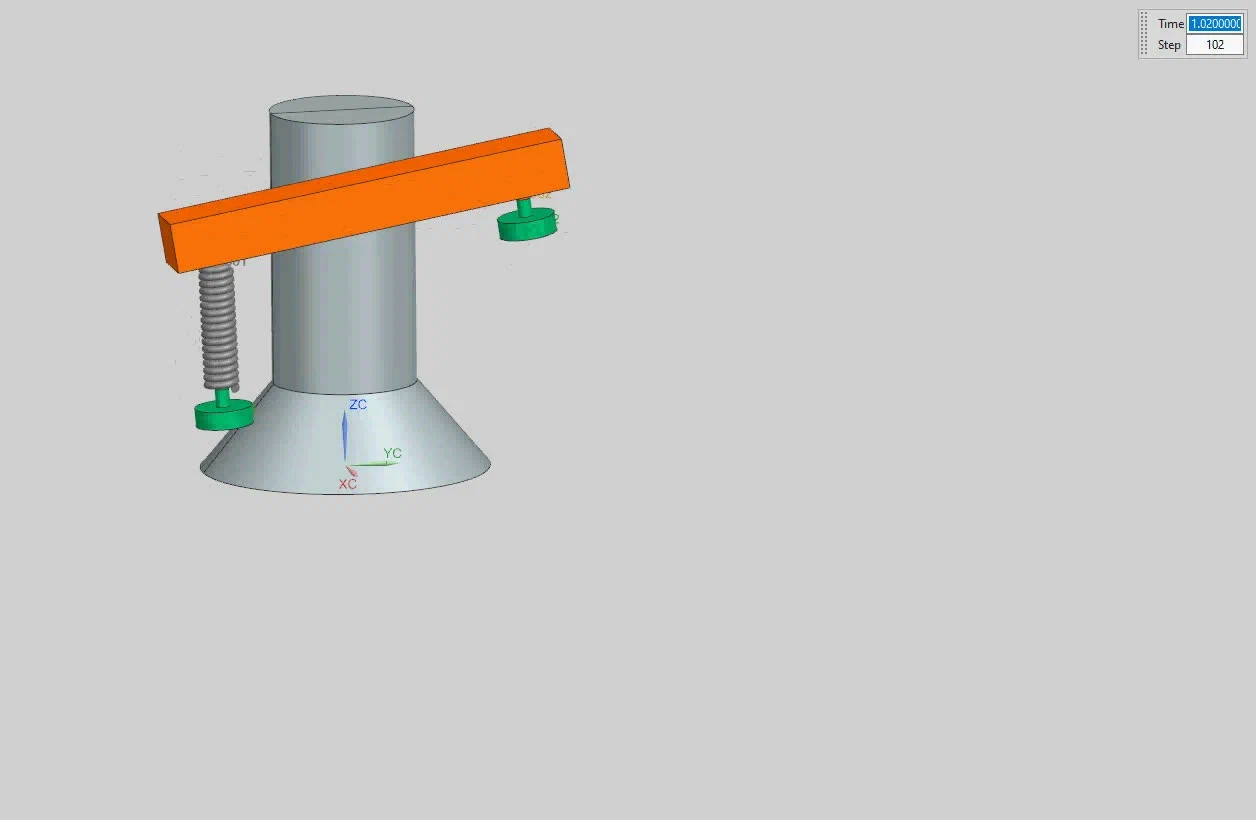
\includegraphics[height=6cm,width=1\textwidth,keepaspectratio]{3_preview.png}}
        % \caption{Click on a picture for a video}
        \label{fig:3_preview.png}
    \end{figure}
\end{frame}

\begin{frame}[t]{Task 4}
    \framesubtitle{Extended Task Description}
    \footnotesize
    \vspace{-0.3cm}

    \textbf{Goals}:
    \begin{enumerate}
        \footnotesize
        \item Plot the vertical displacement of the bottom clamp (fig. \ref{fig:4_3.jpg});
        \item Determine the maximum height to which the bottom collar will rise in 10 seconds;
        \item Determine the maximum angular velocity of the regulator that will occur at 10 seconds.
    \end{enumerate}
    \smallskip

    \textbf{Description}: Construct a geometric model of the centrifugal regulator (fig. \ref{fig:4_1.jpg}). The upper red collar rotates around a center pin, but is fixed at a certain height. The lower collar both rotates and moves at a certain height. All joints of the mechanism should be described by rotational and cylindrical joints.
    \smallskip

    Naturally, under the action of the weight, the weights of the regulator should take a vertical position at the initial moment of time (fig. \ref{fig:4_2.jpg}). But during rotation, the weights of the regulator will lift and take a certain position at an angle to the vertical (fig. \ref{fig:4_1.jpg}).
    
    Set the masses of spherical weights on the order of 5 --- 6 $kg$. Initial distance between collars --- 150 $mm$.

    Upper red collar should rotates with angular acceleration $50\ ^\circ /s^2$. Analysis time --- 10 sec.
\end{frame}

\begin{frame}[t]{Task 4}
    \framesubtitle{Video}
    \vspace{-1cm}
    \begin{figure}[H]
        \begin{subfigure}{0.32\textwidth}
            \centering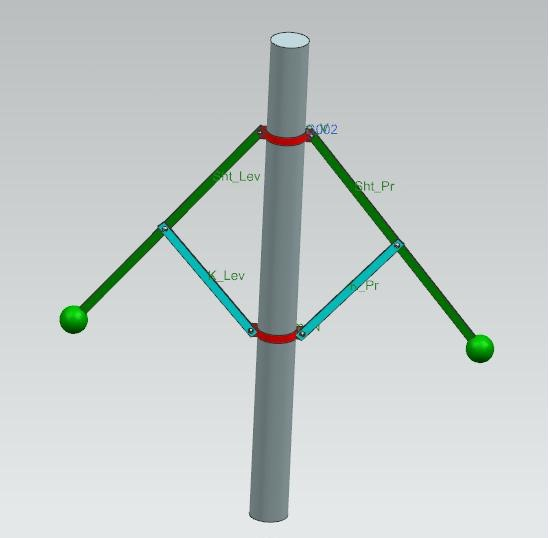
\includegraphics[height=6cm,width=1\textwidth,keepaspectratio]{4_1.jpg}
            \caption{Some particular position}
            \label{fig:4_1.jpg}
        \end{subfigure}
        \begin{subfigure}{0.22\textwidth}
            \centering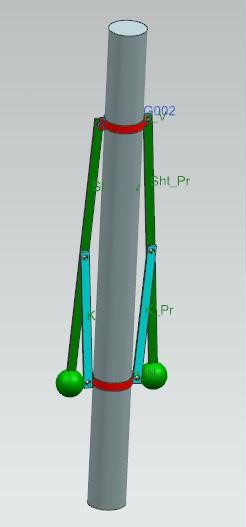
\includegraphics[height=6cm,width=1\textwidth,keepaspectratio]{4_2.jpg}
            \caption{Lowest Position}
            \label{fig:4_2.jpg}
        \end{subfigure}
        \begin{subfigure}{0.42\textwidth}
            \centering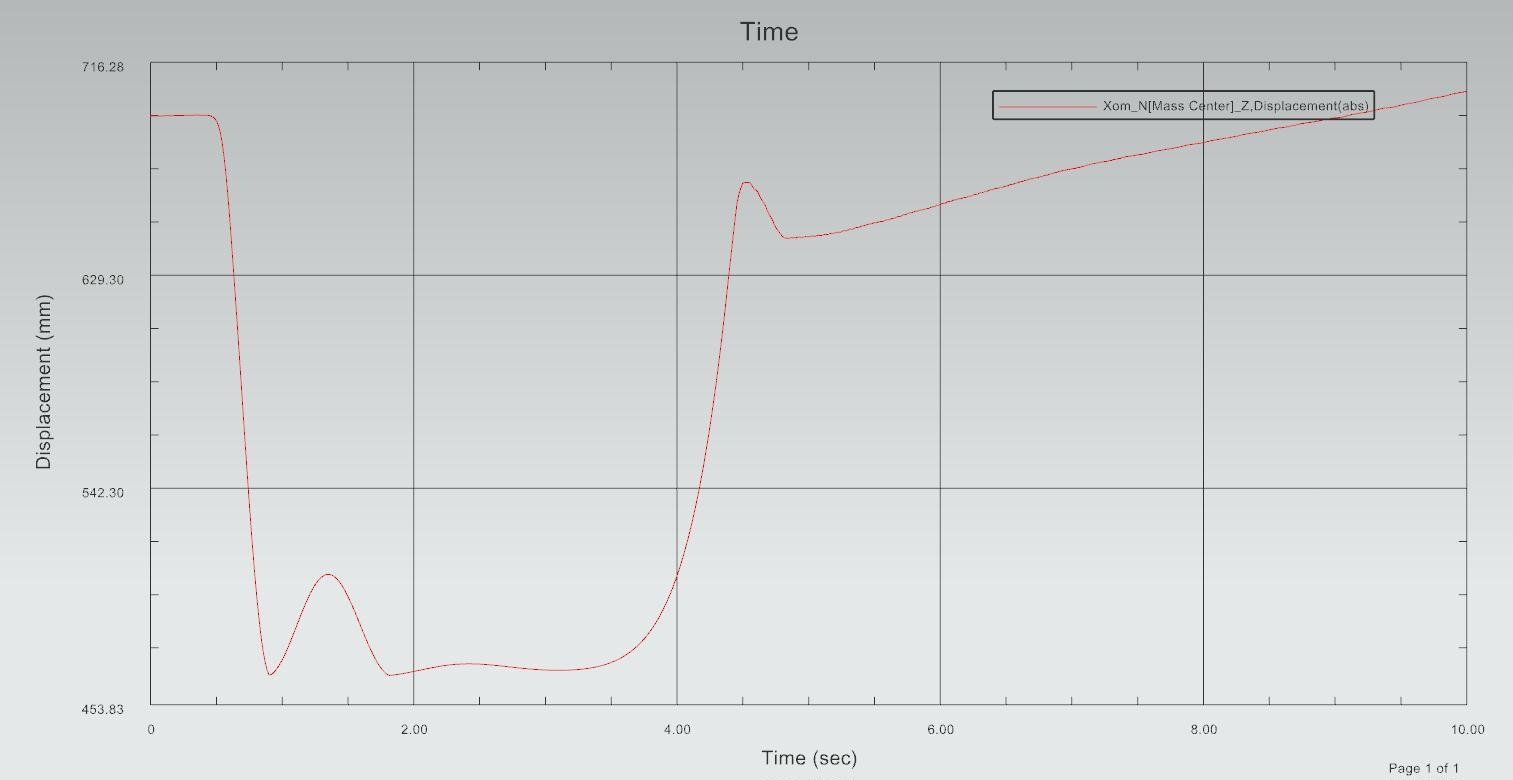
\includegraphics[height=6cm,width=1\textwidth,keepaspectratio]{4_3.jpg}
            \caption{Expected displacement plot (can be not the same)}
            \label{fig:4_3.jpg}
        \end{subfigure}
    \end{figure}
\end{frame}

\fbckg{fibeamer/figs/last_page.png}
\frame[plain]{}

\end{document}